\documentclass{article}
\usepackage[margin=1in]{geometry}
\usepackage{graphicx}
\usepackage{amsmath}
\usepackage{amssymb}

\title{CSCI 567: Homework 1}
\author{anselzen@usc.edu (6163567905) and punyanay@usc.edu (8837304797)}
\date{September 13, 2026}

\begin{document}

\maketitle

\section*{Problem 1}

\subsection*{1.1}

We're asked to find $\nabla_{\mathbf{w}} g(\mathbf{w})$ for
\[
g(\mathbf{w}) = \mathbf{b}^\top \mathbf{w} + \frac{1}{2}\mathbf{w}^\top A \mathbf{w}.
\]

Writing $\mathbf{b}^\top \mathbf{w} = \sum_i b_i w_i$, only the term $b_k w_k$ depends on $w_k$, so
\[
\frac{\partial}{\partial w_k}\sum_i b_i w_i = b_k \quad \text{for every } k,
\]
which gives $\nabla_{\mathbf{w}}(\mathbf{b}^\top \mathbf{w}) = \mathbf{b}$.

\medskip
\noindent
Now for the quadratic piece. Writing $\mathbf{w}^\top A \mathbf{w} = \sum_i \sum_j A_{ij} w_i w_j$,
look at which terms in this double sum actually involve $w_k$: only the terms where $i=k$
or $j=k$. So
\[
\frac{\partial}{\partial w_k}\sum_{i,j} A_{ij} w_i w_j
= \underbrace{\sum_j A_{kj} w_j}_{\text{from } i=k} + \underbrace{\sum_i A_{ik} w_i}_{\text{from } j=k}
= (A\mathbf{w})_k + (A^\top \mathbf{w})_k.
\]
Doing this for every $k$ gives
\[
\nabla_{\mathbf{w}}(\mathbf{w}^\top A \mathbf{w}) = A\mathbf{w} + A^\top\mathbf{w} = (A+A^\top)\mathbf{w}.
\]
Since $A$ is symmetric ($A=A^\top$), this becomes $2A\mathbf{w}$, so
\[
\nabla_{\mathbf{w}}\left(\frac{1}{2}\mathbf{w}^\top A \mathbf{w}\right) = \frac{1}{2}(2A\mathbf{w}) = A\mathbf{w}.
\]

\medskip
\noindent
Adding the two pieces together (gradients add over sums):
\[
\boxed{\nabla g(\mathbf{w}) = \mathbf{b} + A\mathbf{w}}
\]

\subsection*{1.2}

We're asked for the rank of $xx^\top$ when $x \in \mathbb{R}^n$ is nonzero. Look at the columns of $xx^\top \in \mathbb{R}^{n\times n}$: the $(i,j)$ entry is $x_i x_j$, so column $j$ is
\[
(xx^\top)_{:,j} = x_j \cdot x,
\]
i.e.\ every column is just a scalar multiple of the same vector $x$. So all columns live in the one-dimensional span of $x$, which means the rank is at most $1$. Since $x \neq 0$, at least one column is a nonzero multiple of $x$, so the rank is at least $1$ too.
\[
\boxed{\text{rank}(xx^\top) = 1}
\]

\subsection*{1.3}

We're asked to show $\text{tr}(AB) = \text{tr}(BA)$ for $A \in \mathbb{R}^{m\times n}$, $B \in \mathbb{R}^{n \times m}$ (so $AB \in \mathbb{R}^{m \times m}$ and $BA \in \mathbb{R}^{n \times n}$). By definition of matrix multiplication, $(AB)_{ij} = \sum_{k=1}^n A_{ik}B_{kj}$, so
\[
\text{tr}(AB) = \sum_{i=1}^m (AB)_{ii} = \sum_{i=1}^m \sum_{k=1}^n A_{ik}B_{ki}.
\]

\medskip
\noindent
Similarly,
\[
\text{tr}(BA) = \sum_{k=1}^n (BA)_{kk} = \sum_{k=1}^n \sum_{i=1}^m B_{ki}A_{ik}.
\]

\medskip
\noindent
Both double sums range over the same pairs $(i,k)$ with $1 \le i \le m$, $1 \le k \le n$, and involve the same scalar products $A_{ik}B_{ki} = B_{ki}A_{ik}$ (scalar multiplication commutes). Reordering the terms of a finite sum does not change its value, so
\[
\boxed{\text{tr}(AB) = \text{tr}(BA)}
\]

\subsection*{1.4}

We're asked to show $A = \begin{pmatrix} 2 & 1 \\ 1 & 2 \end{pmatrix}$ is positive semidefinite by writing $x^\top A x$ as a sum of squares. Let $x = (x_1, x_2)$. First compute $Ax$ by taking the dot product of each row of $A$ with $x$:
\[
Ax = \begin{pmatrix} 2x_1 + x_2 \\ x_1 + 2x_2 \end{pmatrix}.
\]

\medskip
\noindent
Then
\[
x^\top A x = x_1(2x_1+x_2) + x_2(x_1+2x_2) = 2x_1^2 + 2x_1x_2 + 2x_2^2.
\]

\medskip
\noindent
Using $(x_1+x_2)^2 = x_1^2 + 2x_1x_2 + x_2^2$, we can write
\[
2x_1^2 + 2x_1x_2 + 2x_2^2 = (x_1+x_2)^2 + x_1^2 + x_2^2.
\]
Each term on the right is a square of a real number, hence nonnegative, so $x^\top A x \ge 0$ for every $x \in \mathbb{R}^2$.
\[
\boxed{A \text{ is positive semidefinite}}
\]

\section*{Problem 2}

\subsection*{2.1}
Trained and tested on 2019 movie reviews, but fails on 2026 social media slang. This is
an \textbf{external validity} failure. The model did well on its own
benchmark distribution (2019 reviews), but that distribution doesn't match the
distribution it's actually deployed on (2026 slang-filled posts). Nothing leaked into
training and nobody tuned against a fixed test set. The world the model is being used
on simply changed from the world it was evaluated on.

\subsection*{2.2}
Benchmark answers were sitting on public GitHub before the model's training data was
collected. This is a \textbf{contamination} failure: the test answers probably
ended up inside the pretraining corpus itself, so a high score might just reflect the
model recalling memorized answers rather than actually solving new instances of the
problem.

\subsection*{2.3}
300 tweaks were tried, each kept only if it improved the score on the same public test
set, and the final score ends up noticeably higher than on fresh data. This is
\textbf{IID generalization}, specifically the \textit{adaptive overfitting}
mechanism from lecture. Repeatedly keeping whichever variant scores best on one fixed
test set is basically p-hacking: with enough attempts, some of those "improvements"
are really just noise in that particular test set getting mistaken for real progress,
which is why the score drops on fresh data.

\subsection*{2.4}
A model outscores doctors on a multiple-choice exam, and this gets used to claim it's
ready to diagnose real patients. This is a \textbf{construct validity} failure:
the exam score itself might be totally accurate and uncontaminated, but a multiple-choice
licensing exam and actually diagnosing a real patient (gathering evidence, handling
ambiguity, acting under uncertainty) are just different tasks. Doing well on the narrow
benchmark doesn't automatically support the much bigger claim being made about real-world
readiness.

\section*{Problem 3}

\subsection*{3.1}

We want to find how large the test set $n$ needs to be so the empirical accuracy $\bar{Z}$ lands within
$\varepsilon$ of the true accuracy $\mu$ with probability at least $1-\delta$:
\[
P\big[\,|\bar Z - \mu| < \varepsilon\,\big] \ge 1-\delta,
\]
which is the same as asking the \emph{failure} probability to be small,
\[
P\big[\,|\bar Z - \mu| \ge \varepsilon\,\big] \le \delta.
\]

\medskip
\noindent
Hoeffding's inequality (as stated in lecture) already gives us an upper bound on that failure probability:
\[
P\big[\,|\bar Z - \mu| \ge \varepsilon\,\big] \le 2\exp(-2n\varepsilon^2).
\]

\medskip
\noindent
So it's enough to force this upper bound itself to be at most $\delta$:
\[
2e^{-2n\varepsilon^2} \le \delta.
\]

\medskip
\noindent
Solve for $n$. Divide both sides by 2, then take $\ln$ of both sides:
\[
e^{-2n\varepsilon^2} \le \frac{\delta}{2}
\quad\Longrightarrow\quad
-2n\varepsilon^2 \le \ln\!\left(\frac{\delta}{2}\right).
\]
Now multiply both sides by $-1$ (which flips the inequality direction), and use
$-\ln(\delta/2) = \ln(2/\delta)$:
\[
2n\varepsilon^2 \ge -\ln\!\left(\frac{\delta}{2}\right) = \ln\!\left(\frac{2}{\delta}\right)
\quad\Longrightarrow\quad
\boxed{n \ge \frac{1}{2\varepsilon^2}\ln\!\left(\frac{2}{\delta}\right)}
\]

\medskip
\noindent
\textbf{Plugging in numbers, $\delta = 0.05$:}

Here $\ln(2/0.05) = \ln(40) \approx 3.6889$.

\begin{itemize}
    \item $\varepsilon = 0.01$:
    \[
    n \ge \frac{3.6889}{2(0.01)^2} = \frac{3.6889}{0.0002} \approx 18{,}444.5
    \quad\Longrightarrow\quad
    \boxed{n \ge 18{,}445}
    \]
    \item $\varepsilon = 0.001$:
    \[
    n \ge \frac{3.6889}{2(0.001)^2} = \frac{3.6889}{0.000002} \approx 1{,}844{,}440
    \quad\Longrightarrow\quad
    \boxed{n \ge 1{,}844{,}440}
    \]
\end{itemize}

\medskip
\noindent
\textbf{General lesson.} Since $n \propto 1/\varepsilon^2$, shrinking $\varepsilon$ by a
factor of $10$ (one more decimal digit of certified precision) forces $n$ to grow by a
factor of $10^2 = 100$. That's exactly what happened above: going from $\varepsilon=0.01$
to $\varepsilon=0.001$ multiplied the required sample size by about $100\times$. Precision
gets expensive fast. Each extra digit of certainty costs two orders of magnitude more
data, not just ten times more.

\subsection*{3.2}

\textbf{(i) The two half-widths.}

For each test set $j \in \{1,2\}$, Hoeffding gives a confidence interval
$[A_j-\varepsilon_j,\,A_j+\varepsilon_j]$ that contains $\mu$ with probability at least
$1-\delta_j$, where
\[
\delta_j = 2e^{-2n_j\varepsilon_j^2}.
\]

\medskip
\noindent
This is the same equation as in 3.1, just now we're solving for $\varepsilon_j$ instead of
$n$. Divide by 2 and take $\ln$:
\[
e^{-2n_j\varepsilon_j^2} \le \frac{\delta_j}{2}
\quad\Longrightarrow\quad
-2n_j\varepsilon_j^2 \le \ln\!\left(\frac{\delta_j}{2}\right).
\]
Multiply both sides by $-1$ (flipping the inequality), and again use $-\ln(\delta_j/2)=\ln(2/\delta_j)$:
\[
2n_j\varepsilon_j^2 \ge \ln\!\left(\frac{2}{\delta_j}\right)
\quad\Longrightarrow\quad
\varepsilon_j^2 \ge \frac{1}{2n_j}\ln\!\left(\frac{2}{\delta_j}\right)
\]
\[
\boxed{\varepsilon_j = \sqrt{\frac{\ln(2/\delta_j)}{2n_j}}}
\]

\medskip
\noindent
At $95\%$ confidence, $\delta_j = 0.05$ for both test sets, so $\ln(2/\delta_j) \approx 3.6889$ in both cases.

\begin{itemize}
    \item $n_1 = 50{,}000$:
    \[
    \varepsilon_1 = \sqrt{\frac{3.6889}{2(50{,}000)}} = \sqrt{\frac{3.6889}{100{,}000}} \approx \sqrt{3.689\times 10^{-5}} \approx 0.00607
    \]
    \[
    \boxed{\varepsilon_1 \approx 0.61\%}
    \]
    \item $n_2 = 10{,}000$:
    \[
    \varepsilon_2 = \sqrt{\frac{3.6889}{2(10{,}000)}} = \sqrt{\frac{3.6889}{20{,}000}} \approx \sqrt{1.844\times 10^{-4}} \approx 0.01358
    \]
    \[
    \boxed{\varepsilon_2 \approx 1.36\%}
    \]
\end{itemize}

\medskip
\noindent
The smaller test set gives a wider (less certain) interval, which makes sense: less data
means less confidence about where $\mu$ actually is.

\bigskip
\noindent
\textbf{(ii)(a) Simultaneous validity fails with probability at most $\delta_1+\delta_2$.}

\medskip
\noindent
Let $F_j$ be the event that interval $j$ \emph{fails} to contain $\mu$; by construction
$P[F_j] \le \delta_j$. "Simultaneous validity" means both intervals contain $\mu$, i.e.\
neither $F_1$ nor $F_2$ happens.

\medskip
\noindent
By the union bound,
\[
P[F_1 \cup F_2] \le P[F_1] + P[F_2] \le \delta_1 + \delta_2.
\]

\medskip
\noindent
Since "simultaneous validity fails" is exactly the event $F_1 \cup F_2$,
\[
\boxed{P[\text{simultaneous validity fails}] \le \delta_1 + \delta_2}
\]

\bigskip
\noindent
\textbf{(ii)(b) Simultaneous validity forces the intervals to overlap.}

\medskip
\noindent
Suppose both intervals do contain $\mu$: $|A_1 - \mu| \le \varepsilon_1$ and
$|A_2-\mu|\le \varepsilon_2$.

\medskip
\noindent
By the triangle inequality,
\[
|A_1 - A_2| = \big|(A_1-\mu) - (A_2-\mu)\big| \le |A_1-\mu| + |A_2-\mu| \le \varepsilon_1+\varepsilon_2.
\]
\[
\boxed{|A_1-A_2| \le \varepsilon_1+\varepsilon_2}
\]

\medskip
\noindent
So whenever both confidence intervals are correct, the two measured accuracies $A_1$ and
$A_2$ can't be farther apart than the sum of their half-widths. That's exactly the
condition for the two intervals to overlap on the real line. If the observed gap
$|A_1-A_2|$ is much bigger than $\varepsilon_1+\varepsilon_2$, that's strong evidence the
two test sets aren't just noisy measurements of the same true accuracy $\mu$.

\section*{Problem 4:}
\subsection*{4.1}

Let $I \in \{1, \ldots, n\}$ be drawn uniformly.

For an i.i.d $X$,
\[
\mathbb{E}[X] = \sum_i P(x_i) \cdot x_i
\]

For $\mathbb{E}[\mathbf{g}_I]$:
\[
\mathbb{E}[\mathbf{g}_I] = \sum_i P(I=i) \cdot \mathbf{g}_i
\]

For an i.i.d, $P(I=i) = \frac{1}{n}$
\[
\mathbb{E}[\mathbf{g}_I] = \sum_i \frac{1}{n} \mathbf{g}_i = \frac{1}{n}\sum_i \mathbf{g}_i = \nabla \hat{R}(\mathbf{w}) = \mathbf{g}
\]

Similarly,
\[
\mathbb{E}\big[\|\mathbf{g}_i - \mathbf{g}\|^2\big] = \sum_i P(I=i) \|\mathbf{g}_i - \mathbf{g}\|^2 = \frac{1}{n}\sum_i \|\mathbf{g}_i - \mathbf{g}\|^2 = \sigma^2
\]

\subsection*{4.2}

$B$ indices i.i.d $I_1, \ldots, I_B$

\[
\hat{\mathbf{g}}_B = \frac{1}{B}\sum_{b=1}^B \mathbf{g}_{I_b}
\]

\[
\mathbb{E}[\hat{\mathbf{g}}_B] = \frac{1}{B}\sum_{b=1}^B \mathbb{E}[\mathbf{g}_{I_b}] = \frac{1}{B} B \cdot \mathbf{g} = \mathbf{g}
\]

\[
\hat{\mathbf{g}}_B - \mathbf{g} = \frac{1}{B}\sum_{b=1}^B \mathbf{g}_{I_b} - \frac{1}{B}\sum_b \mathbf{g} = \frac{1}{B}\sum_b (\mathbf{g}_{I_b} - \mathbf{g})
\]

\[
\|\hat{\mathbf{g}}_B - \mathbf{g}\|^2 = \frac{1}{B^2}\sum_{b=1}^B \sum_{c=1}^B (\mathbf{g}_{I_b} - \mathbf{g})^T (\mathbf{g}_{I_c} - \mathbf{g})
\]

\[
\mathbb{E}\big[\|\hat{\mathbf{g}}_B - \mathbf{g}\|^2\big] = \frac{1}{B^2}\sum_{b=1}^B \sum_{c=1}^B \mathbb{E}\big[(\mathbf{g}_{I_b} - \mathbf{g})^T (\mathbf{g}_{I_c} - \mathbf{g})\big]
\]

When $b = c$:
\[
\mathbb{E}\big[\|\mathbf{g}_{I_b} - \mathbf{g}\|^2\big] = \sigma^2
\]

When $b \ne c$:
\[
\mathbb{E}\big[(\mathbf{g}_{I_b} - \mathbf{g})^T (\mathbf{g}_{I_c} - \mathbf{g})\big] = \mathbb{E}[(\mathbf{g}_{I_b} - \mathbf{g})(\mathbf{g}_{I_c} - \mathbf{g})^T] = 0
\]

$\Rightarrow b = c$ for $B$ terms
\[
\mathbb{E}\big[\|\hat{\mathbf{g}}_B - \mathbf{g}\|^2\big] = \frac{1}{B^2} \cdot B \sigma^2 = \frac{\sigma^2}{B}
\]

\section*{Problem 5:}
\subsection*{5.1 Closed Form}

\begin{itemize}
    \item[(i)]   $\hat{\mathcal{R}}(\mathbf{w}_{LS}) = 0.117523$
    \item[(ii)]  $\hat{\mathcal{R}}(\mathbf{0}) = 37.6633$
    \item[(iii)] $\hat{\mathcal{R}}_{\text{test}}(\mathbf{w}_{LS}) = 0.139395$
\end{itemize}

The test risk is higher than the train risk because $\mathbf{w}_{LS}$ is chosen
specifically to minimize the training loss, so it fits the noise particular to
the training sample rather than the true underlying signal.

The training risk is lower than the noise floor because, with $D$ dimensions
relative to $N$ samples, the model overfits, causing it to absorb part of the
training noise and pulling the training risk below the noise floor. Based on
the noise floor $\mathrm{Var}[\varepsilon]/2 = 0.125$, the training risk is
approximately $0.9 \times 0.125$, and the test risk is approximately
$1.1 \times 0.125$.

\subsection*{5.2 Gradient Descent}

\begin{figure}[h]
    \centering
    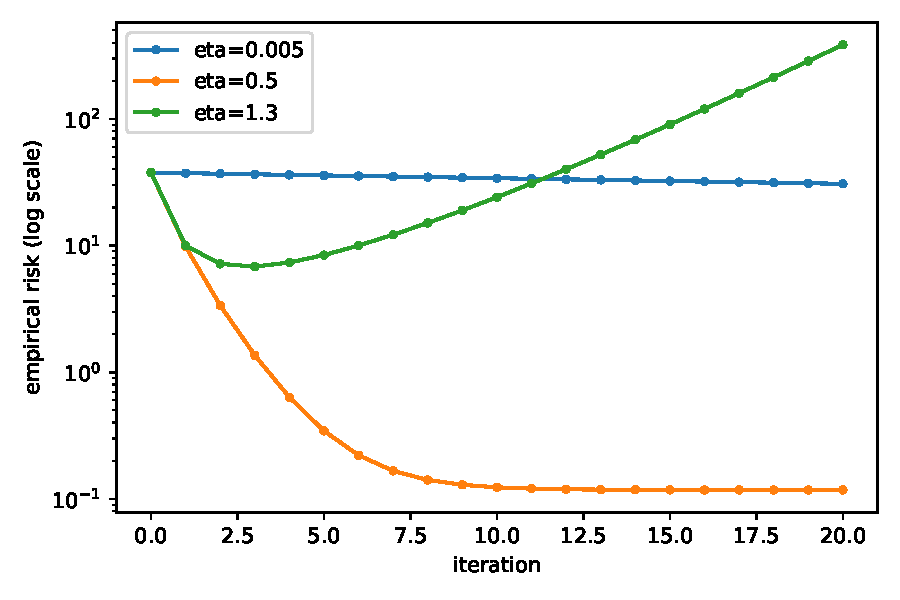
\includegraphics[width=0.8\textwidth]{gd_curves.pdf}
    \caption{Empirical risk vs.\ iteration for gradient descent, $\eta \in \{0.005, 0.5, 1.3\}$.}
    \label{fig:gd_curves}
\end{figure}

\begin{itemize}
    \item GD $\eta = 0.005$: final $\hat{\mathcal{R}} = 30.7255$
    \item GD $\eta = 0.5$: final $\hat{\mathcal{R}} = 0.117533$
    \item GD $\eta = 1.3$: final $\hat{\mathcal{R}} = 384.81$
\end{itemize}

For $\eta = 0.005$, the empirical risk on the log-scale plot stays almost the
same, which means that at each iteration the gradient step is extremely
small and moves slowly toward the optimal point, i.e., the step size is too
small.

For $\eta = 0.5$, we get a training loss that gradually moves toward the
optimal point, the kind of gradual loss decrease we want.

For $\eta = 1.3$, instead of stepping toward the global minimum, since the
step size is so large, each update overshoots further past the minimum than
the previous step did, causing the loss to shoot up with the number of
iterations.

\subsection*{5.3 SGD}

\begin{figure}[h]
    \centering
    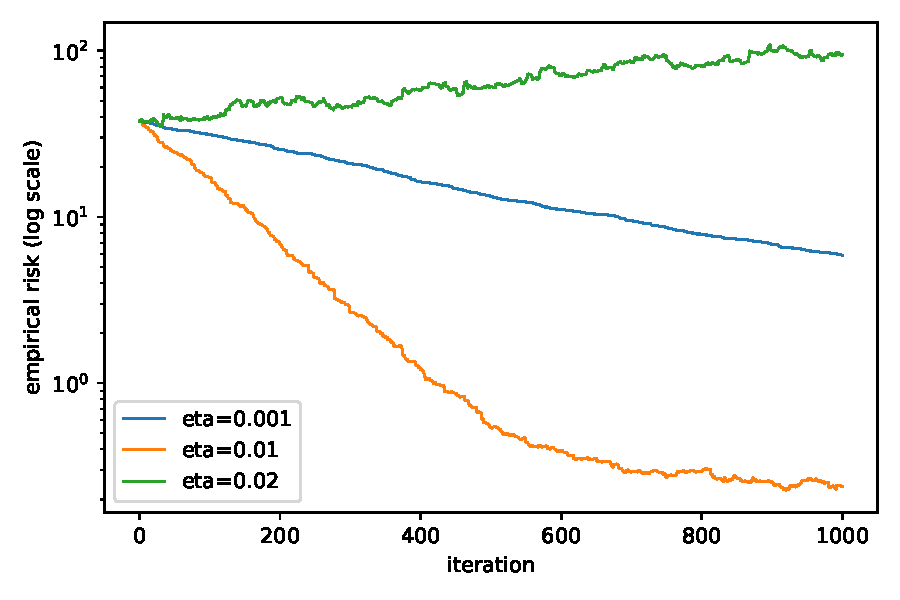
\includegraphics[width=0.8\textwidth]{sgd_curves.pdf}
    \caption{Empirical risk vs.\ iteration for SGD, $\eta \in \{0.001, 0.01, 0.02\}$.}
    \label{fig:sgd_curves}
\end{figure}

\begin{itemize}
    \item SGD $\eta = 0.001$: final $\hat{\mathcal{R}} = 5.886$
    \item SGD $\eta = 0.01$: final $\hat{\mathcal{R}} = 0.23842$
    \item SGD $\eta = 0.02$: final $\hat{\mathcal{R}} = 94.3621$
\end{itemize}

For $\eta = 0.001$, the loss moves very slowly toward the optimal solution.
For $\eta = 0.01$, the loss moves gradually toward the optimum value as
expected. For $\eta = 0.02$, the model overshoots, and the loss keeps
moving away from the optimum with each iteration.

Since GD evaluates all $N = 1000$ data points per step, while SGD evaluates
one randomly drawn data point per step, GD uses far more data per
iteration: each GD step requires 1000 gradient evaluations, compared to 1
for SGD. Over the full run, GD performs 20 steps $\times$ 1000 examples
$=$ 20 epochs over the data, whereas SGD performs 1000 steps $\times$ 1
example $=$ roughly 1 epoch over the data. SGD's curve is jagged because
the gradient estimate from a single data point has much higher variance
than the gradient computed over the entire dataset, so individual steps do
not consistently decrease the full-batch risk. GD reaches the lower
objective in this experiment ($\hat{\mathcal{R}} = 0.117533$ at
$\eta = 0.5$, versus $0.23842$ for SGD's best case at $\eta = 0.01$),
despite touching far less data per step, because it performs many more
total passes over the dataset (20 epochs vs. roughly 1).


\end{document}